\paragraph{QuizziPedia::Front-End::Models::QuestionItemModel}
		
		\label{QuizziPedia::Front-End::Models::QuestionItemModel}
		
		\begin{figure}[ht]
			\centering
			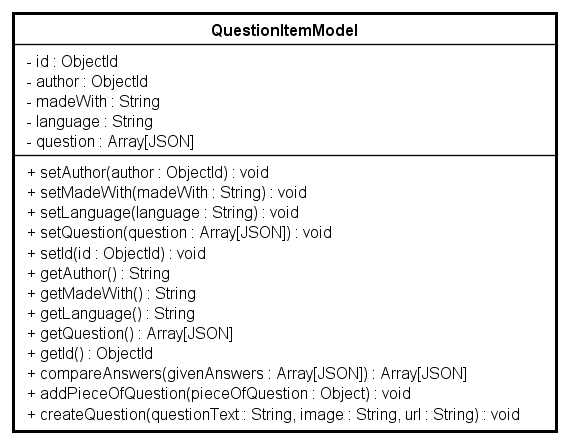
\includegraphics[scale=0.5,keepaspectratio]{UML/Classi/Front-End/QuizziPedia_Front-end_Models_QuestionItemModel.png}
			\caption{QuizziPedia::Front-End::Models::QuestionItemModel}
		\end{figure} \FloatBarrier
		
		\begin{itemize}
			\item \textbf{Descrizione}: rappresenta una domanda. Contiene tutte le informazioni necessarie alla presentazione del contenuto della domanda;
			\item \textbf{Utilizzo}: viene utilizzata per memorizzare i dati di una domanda;
			\item \textbf{Relazioni con altre classi}: 
			\begin{itemize}
				\item \textit{OUT} \texttt{QuestionsManagementController}: questa classe permette di gestire e di ottenere le domande create dall'utente;
				\item \textit{IN} \texttt{TrueFalseQuestionsController}: questa classe permette di gestire la creazione e la modifica di una domanda vero/falso;
				\item \textit{OUT} \texttt{MultipleQuestionsController}: questa classe permette di gestire la creazione e la modifica di una domanda a risposta multipla; 
				\item \textit{OUT} \texttt{ConnectionQuestionsController}: questa classe permette di gestire la creazione e la modifica di una domanda a collegamento;
				\item \textit{OUT} \texttt{ImagesSortingQuestionsController}: questa classe permette di gestire la creazione e la modifica di una domanda a ordinamento immagini;
				\item \textit{OUT} \texttt{StringsSortingQuestionsController}: questa classe permette di gestire la creazione e la modifica di una domanda a ordinamento di stringhe;
				\item \textit{OUT} \texttt{FillingQuestionsController}: questa classe permette di gestire la creazione e la modifica di una domanda a riempimento di spazi; 
				\item \textit{OUT} \texttt{ClickableAreaQuestionsController}: questa classe permette di gestire la creazione e la modifica di una domanda ad area cliccabile;
				\item \textit{OUT} \texttt{EditorQMLController}: questa classe permette di gestire la creazione e la modifica di domande create tramite editor QML;
				\item \textit{OUT} \texttt{QuestionsController}: questa classe permette di gestire il recupero delle domande per poterle stampare nella modalità allenamento e nei questionari;
			\end{itemize}
			\item \textbf{Attributi}: 
			\begin{itemize}
				\item \texttt{- id: ObjectId}\\
				Rappresenta l'attributo id della domanda. Viene utilizzato solamente dalle domande recuperate dal database;
				\item \texttt{- author: ObjectId}\\
				Rappresenta il riferimento all'identificativo dell'utente che ha creato la domanda;
				\item \texttt{- madeWith: String}\\ 
				Rappresenta con quale strumento è stata creata la domanda;
				\item \texttt{- language: String}\\
				Rappresenta la lingua in cui è scritta la domanda; 
				\item \texttt{- question: Array[JSON]}\\ 
				Contiene un oggetto di tipo \texttt{JSON}. L'oggetto \texttt{JSON} è rappresentato dai seguenti campi:
				\begin{itemize}
					\item \texttt{- type: String}\\
					Rappresenta la tipologia di domanda;
					\item \texttt{- questionText: String}\\ 
					Rappresenta il testo della domanda; 
					\item \texttt{- image: String}\\
					Rappresenta l'\textit{URL\ped{G}} dell'immagine associata al testo della domanda; 
					\item \texttt{- answers: Array[JSON]}\\ 
					Contiene un oggetto di tipo \texttt{JSON}. L'oggetto \texttt{JSON} è rappresentato dai seguenti campi:
					\begin{itemize}	 				  
						\item \texttt{- text: String}\\
						Rappresenta il testo della risposta;
						\item \texttt{- url: String}\\
						Rappresenta l'immagine della risposta;
						\item \texttt{attributesForTForMultiple: Mixed}\\
						Contiene i seguenti attributi:
						\begin{enumerate}
							\item \texttt{- isItRight: Boolean}\\
							Rappresenta se una risposta è giusta o sbagliata.
						\end{enumerate}      
						\item \texttt{- attributesForSorting: Mixed}\\
						Contiene i seguenti attributi:
						\begin{enumerate}
							\item \texttt{- position: Boolean}\\
							Rappresenta quale è la giusta posizione di un testo o immagine all'interno di un esercizio di ordinamento.
						\end{enumerate}  
						\item \texttt{- attributesForLinking: Mixed}\\
						Contiene i seguenti attributi:
						\begin{enumerate}
							\item \texttt{- text1: String}\\
							Rappresenta il primo elemento testuale che deve essere collegato con il secondo elemento testuale o rappresentato da un'immagine;
							\item \texttt{- text2: String}\\
							Rappresenta il secondo elemento testuale che deve essere collegato con il primo elemento testuale o rappresentato da un'immagine;
							\item \texttt{- url1: String}\\
							Rappresenta il primo elemento rappresentato da un'immagine che deve essere collegato con il secondo elemento testuale o rappresentato da un'immagine;
							\item \texttt{- url2: String}\\
							Rappresenta il secondo elemento rappresentato da un'immagine che deve essere collegato con il primo elemento testuale o rappresentato da un immagine.
						\end{enumerate}  
						\item \texttt{- attributesForClickableArea: Mixed}\\
						Contiene i seguenti attributi:
						\begin{enumerate}
							\item \texttt{- x: Number}\\
							Rappresenta la coordinata x di una area cliccabile;  
							\item \texttt{- y: Number}\\
							Rappresenta la coordinata y di una area cliccabile. 
						\end{enumerate}    
						\item \texttt{- attributesForEmptySpaces: Mixed}\\
						Contiene i seguenti attributi:
						\begin{enumerate}
							\item \texttt{- wordNumber: Number}\\
							Rappresenta la posizione dello spazio vuoto in cui deve andare inserita la parola.  
						\end{enumerate}        						  						
					\end{itemize}
				\end{itemize}			
			\end{itemize}
			\item \textbf{Metodi}: 
			\begin{itemize}
				\item \texttt{+ setAuthor(author: ObjectId): void} \\
				Metodo \textit{setter\ped{G}} per il campo dati \texttt{author}\\
				\textbf{Parametri}:
				\begin{itemize}
					\item {author: ObjectId}\\
					Questo parametro rappresenta l'autore che ha creato la domanda.
				\end{itemize}
				
				\item \texttt{+ setMadeWith(madeWith: String): void} \\
				Metodo \textit{setter\ped{G}} per il campo dati \texttt{madeWith}\\
				\textbf{Parametri}:
				\begin{itemize}
					\item {madeWith: String}\\
					Questo parametro rappresenta con quale strumento è stata creata la domanda.
				\end{itemize}
				
				\item \texttt{+ setLanguage(language: String): void} \\
				Metodo \textit{setter\ped{G}} per il campo dati \texttt{language}\\
				\textbf{Parametri}:
				\begin{itemize}
					\item {language: String}\\
					Questo parametro rappresenta la lingua della domanda.
				\end{itemize}
				
				\item \texttt{+ setQuestion(question: Array[JSON]): void} \\
				Metodo \textit{setter\ped{G}} per il campo dati \texttt{question}\\
				\textbf{Parametri}:
				\begin{itemize}
					\item {question: Array[JSON]}\\
					Questo parametro rappresenta l'oggetto JSON contenente le parti che compongono la totalità della domanda.
				\end{itemize}
				
				\item \texttt{+ setId(id: ObjectId): void} \\
				Metodo \textit{setter\ped{G}} per il campo dati \texttt{id}\\
				\textbf{Parametri}:
				\begin{itemize}
					\item {id: ObjectId}\\
					Questo parametro rappresenta l'id della domanda.
				\end{itemize}
				
				\item \texttt{+ getAuthor(): String} \\
				Metodo \textit{getter\ped{G}} per il campo dati \texttt{author};
				
				\item \texttt{+ getMadeWith(): String} \\
				Metodo \textit{getter\ped{G}} per il campo dati \texttt{madeWith};
				
				\item \texttt{+ getLanguage(): String} \\
				Metodo \textit{getter\ped{G}} per il campo dati \texttt{language};

				\item \texttt{+ getQuestion(): Array[JSON]} \\
				Metodo \textit{getter\ped{G}} per il campo dati \texttt{question};
				
				\item \texttt{+ getId(): ObjectId} \\
				Metodo \textit{getter\ped{G}} per il campo dati \texttt{id};
				
				\item \texttt{+ compareAnswers(givenAnswers: Array[JSON]): Array[JSON]} \\
				Metodo che compara le risposte date con quelle corrette. Ritorna un \texttt{array} contenente un valore booleano, che indica se è giusta o meno una domanda, per ogni pezzo di domanda che compone la domanda. \\
				\textbf{Parametri}:
				\begin{itemize}
					\item {givenAnswers: Array[JSON]}\\
					Questo parametro contiene le risposte date dall'utente. 
				\end{itemize}
				
				\item \texttt{+ addPieceOfQuestion(pieceOfQuestion: Object): void} \\
				Metodo che permette di inserire un pezzo di domanda all'attributo \texttt{question}.\\
				\textbf{Parametri}:
				\begin{itemize}
					\item {pieceOfQuestion: Object}\\
					Questo parametro rappresenta un pezzo di domanda.
				\end{itemize}
				
				\item \texttt{+ CreateQuestion(questionText: String, image: String, url: String): void} \\
				Metodo che inizializza il campo \texttt{question}.\\
				\textbf{Parametri}:
				\begin{itemize}
					\item {questionText: String}\\
					Rappresenta il testo della domanda;
					\item {image: String}\\
					Rappresenta l'\textit{URL\ped{G}} dell'immagine associata al testo della domanda. 
				\end{itemize}	
			\end{itemize}
		\end{itemize}
		
		